\section{Supporting Diagnostics}
\label{app:historical_diagnostics}
The following analyses retain historical selector diagnostics and secondary
checks. Main module ablations and the receipt and contract tests remain in
the experimental section.

\paragraph{Useful edits in the earlier selector.}

We use saved proposals and trial graphs from the earlier selector.
These runs came before the shared-feature and candidate-start changes in
Table~\ref{tab:math_revision_selector}. For each document, we try every
subset of model edit bundles and score its graph against the reference.
We apply the saved edits with stopping, cost, and graph-bound checks turned
off. We call the best reference-scored subset the oracle.
This analysis uses model bundles and reference values.

We try 2,144 subsets across 450 inputs.
Table~\ref{tab:selection_bottlenecks} lists the results.
On added-defect inputs, 86 graphs have zero detected violations.
Of these, 72 miss reference fields and 70 have a proposal subset that raises
F1. Among the checked trials, 212 raise reference F1 but have scores of zero
or less. The matching model-built counts are 8 graphs and 1 trial.

\begin{table}[t]
\centering
\caption{Earlier selector results on 225 inputs per group. The oracle uses references to find the best saved subset. One document can have several trials.}
\label{tab:selection_bottlenecks}
\small
\begin{tabular}{lrr}
\toprule
Diagnostic & Controlled & Natural \\
\midrule
Preprocessed graph F1 & 0.8472 & 0.8799 \\
Uniform optimizer F1 & 0.8472 & 0.8833 \\
Fixed-proposal oracle F1 & 0.9964 & 0.9173 \\
Initially no detected violation & 86 & 198 \\
Imperfect among those graphs & 72 & 50 \\
Improvement available among those graphs & 70 & 8 \\
Improving trials with non-positive utility & 212 & 1 \\
\bottomrule
\end{tabular}
\end{table}

Removing edit cost raises F1 on 67 added-defect documents, keeps it the same
on 158, and lowers it on 0. On model-built inputs, it raises F1 on 0,
keeps it the same on 222, and lowers it on 3.
The three graphs with lower F1 already differ from the reference after
cleanup. All 148 exact model-built inputs keep their F1.
The paired added-defect gain is 4.58 points
(95\% document-bootstrap CI: 3.69--5.54).
The same cost change has different effects on the two input groups.


\subsection{Diagnostic Batch Scaling}
\label{sec:eval:scale}

We time the input-derived diagnostic report in
Eq.~(\ref{eq:diagnostic_context}) on disjoint batches containing 1K--50K
triples. A full pass visits every document; a local update recomputes one
changed document. Full times are medians of seven runs and local times of
200 runs. Table~\ref{tab:diagnostic_scaling} reports the measurements.
The memory figure is peak new Python allocation for batch construction,
with source text and schema objects shared. The measured operations are
diagnostic construction and updates; model calls are timed separately.

\begin{figure}[t]
\centering
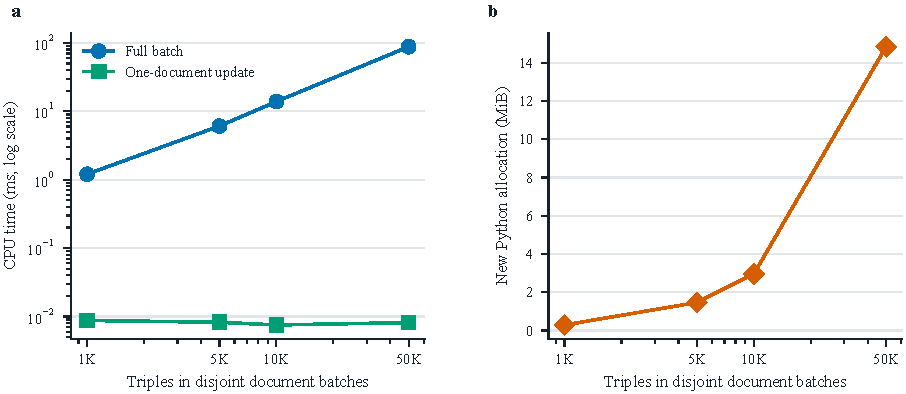
\includegraphics[width=0.98\textwidth]{figure/experiments/diagnostic_scaling.pdf}
\caption{Scaling of input-derived diagnostics on disjoint document batches.
Local updates recompute one document. Memory records new batch allocations
with shared source text.}
\label{fig:diagnostic_scaling}
\end{figure}

\subsection{Secondary Checks}
\label{sec:eval:external_benchmark}

An independent Gemma judge evaluates 180 source--triple pairs without method
identity. Its source-support score correlates with exact reference validity at
Pearson $r=0.794$ and Spearman $\rho=0.807$ (both
$p<2.4\times10^{-40}$). A fixed 50-item subset produces the same mean, 0.96,
in five additional runs. This measures repeatability of the model judge.

We also compare the extraction path with Neo4j Labs' reproducible
\texttt{LLMGraphTransformer} core on 45 balanced TNEWS documents
\citep{ref_neo4j_llm_graph_builder}. Category accuracy is 0.556 for our
schema-guided extractor and 0.533 for Graph Builder; paired outcomes do not
differ ($p=1.00$). TNEWS has no gold triples, so this supports only comparable
behavior under that extraction protocol.


\subsection{Supporting Cost and Scaling Tables}
\begin{table*}[t]
\centering
\caption{Final-run request costs. Means include retries and rate-pacing waits; source preparation and executor queue time are excluded.}
\label{tab:matched_cost}
\small
\resizebox{\textwidth}{!}{%
\begin{tabular}{llrrrr}
\toprule
Input & Context & Calls & Input tokens & Output tokens & Wall (s) \\
\midrule
Controlled & Base & 1.00 & 947 & 517 & 8.58 \\
Controlled & Diagnostic & 1.00 & 1017 & 512 & 8.61 \\
Controlled & SHACL & 1.00 & 3080 & 513 & 8.45 \\
Natural & Base & 1.00 & 832 & 458 & 7.51 \\
Natural & Diagnostic & 1.00 & 901 & 462 & 7.90 \\
Natural & SHACL & 1.00 & 2822 & 455 & 8.16 \\
\bottomrule
\end{tabular}%
}
\end{table*}
\begin{table*}[t]
\centering
\caption{Input-derived diagnostic scaling. Memory is peak new batch allocation in MiB; source texts are shared.}
\label{tab:diagnostic_scaling}
\small
\resizebox{\textwidth}{!}{%
\begin{tabular}{rrrrr}
\toprule
Triples & Documents & Full (ms) & Local (ms) & Allocation (MiB) \\
\midrule
1,000 & 143 & 1.20 & 0.009 & 0.29 \\
5,000 & 716 & 6.08 & 0.008 & 1.47 \\
10,000 & 1,434 & 13.90 & 0.008 & 2.96 \\
50,000 & 7,173 & 88.10 & 0.008 & 14.84 \\
\bottomrule
\end{tabular}%
}
\end{table*}

